\subsection{Volume of Fluid (VOF)}
\label{sec:vof}

O método \textit{Volume of Fluid} é pertencente à família dos métodos de captura de interface, formulado segundo a abordagem de um único fluido (\textit{one-fluid}) que resolve um conjunto de equações para ambas as fases, com a interface entre elas sendo definida por uma função de volume de fluido. Foi primeiramente apresentado por \citet{Hirt1981} cuja ideia de representar a interface por uma fração volumétrica já estava presente em métodos anteriores, como o \textit{SLIC} de \citet{Noh1976}. O método \textit{VOF} é amplamente utilizado devido sua versatilidade, robustez e capacidade de lidar com problemas de interface e topologias complexas, com grandes deformações, além de conservar massa e volume. Enquanto algums das equações mostradas abaixo para exemplificar a $VOF$ são os mesmos utilizados no código base para o desenvolvimento do presente trabalho, uma recente revisão mais detalhada do estado da arte do mesmo pode ser encontrado em \citet{Mohan2024}. A Figura \ref{fig:vof-esquema} mostra um esquema do que foi utilizado localmente.

\begin{figure}
    \centering
    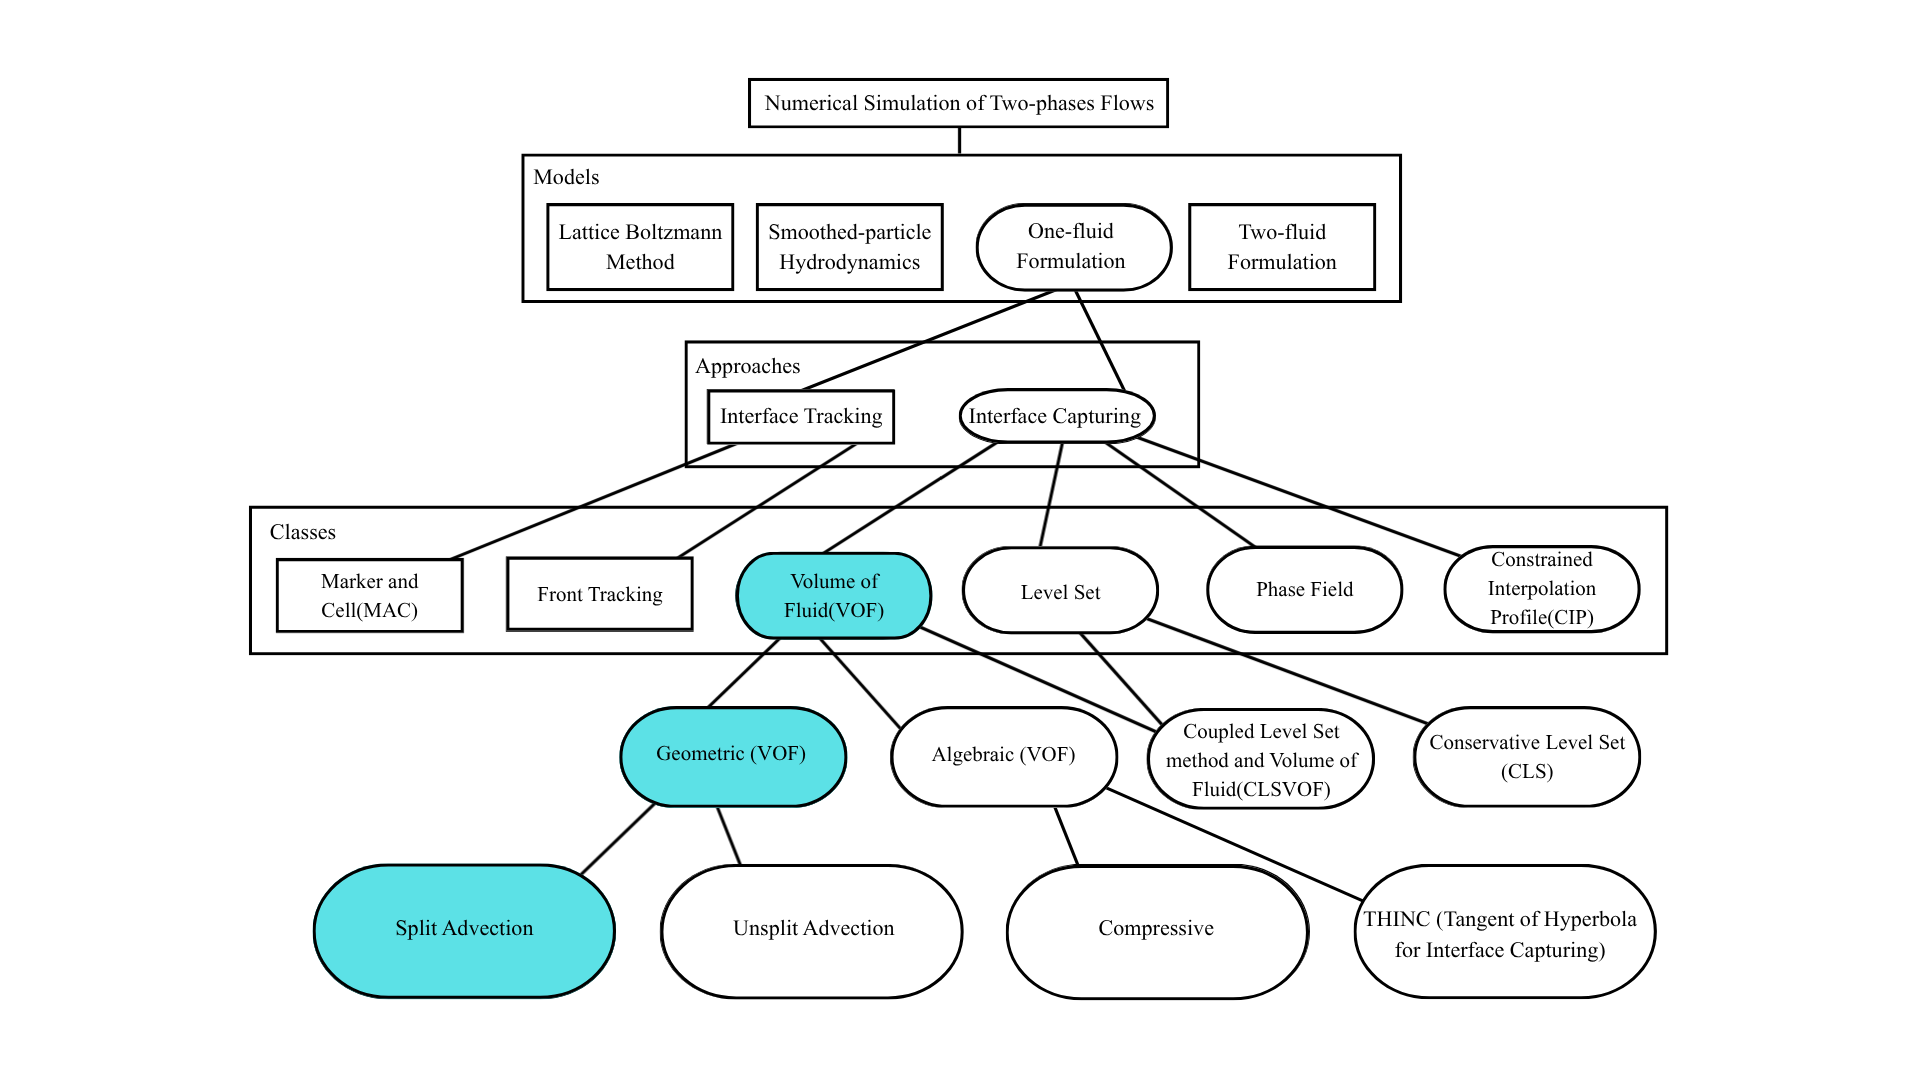
\includegraphics[width=1\textwidth]{imagens/vof-esquema-maria.png}
    \caption{Esquema do método \textit{VOF} utilizado no presente trabalho (adaptado de \citet{Mohan2024}).}
    \label{fig:vof-esquema}
\end{figure}

A função coloração é, or definição, descontínua na interface. Sendo assim faz-se necessário o uso de uma função auxiliar para que seja possível calcular as derivadas nas funções de transporte da mesma, essa função auxiliar é chamada de fração volumétrica $f$, média de $c$ no volume da célula \citep{Weymouth2010}, Eq \ref{eq:fraction-vof}

\begin{equation}
    f = \frac{1}{V} \int_V c dV,
    \label{eq:fraction-vof}
\end{equation}

de modo que $f = 1$ nas células ocupadas pelo fluido 1, $f = 0$ nas ocupadas
pelo fluido 2 e $0 < f < 1$ nas células atravessadas pela interface, como
ilustra a Figura~\ref{fig:vof-exemplo}. A posição da interface no interior de
cada célula não é armazenada, e sim reconstruída a partir do campo de $f$.

\begin{figure}
    \centering
    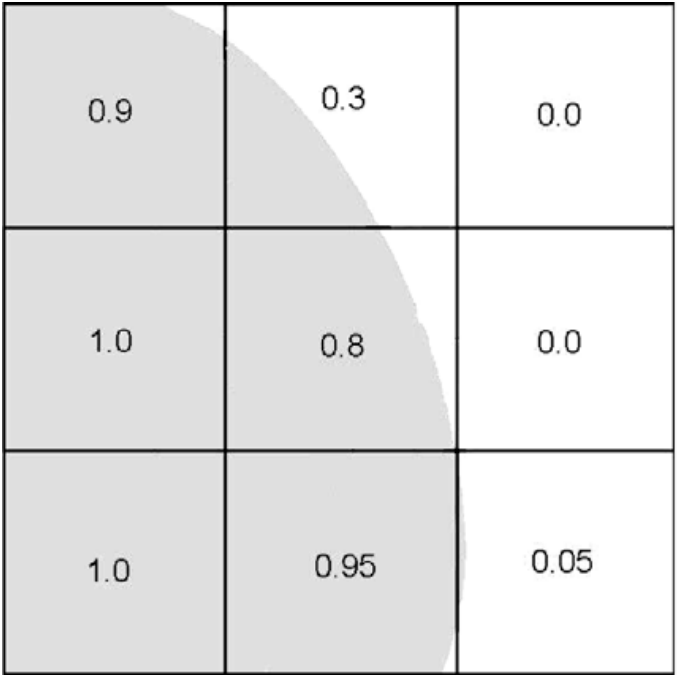
\includegraphics[width=0.5\textwidth]{imagens/vof-grid-weymouth.png}
    \caption{Exemplo de como a função coloração representa ambos os fluidos (adaptada de \citet{Weymouth2010}).}
    \label{fig:vof-exemplo}
\end{figure}


A fração volumétrica é transportada em forma de fluxos, sendo que todo o volume do fluido 1 que deixa uma célula é incorporado na célula vizinha, atendendo assim as equações de balanço discretas. Em esquemas com separação direcional, nos quais a advecção é decomposta em varreduras unidimensionais sucessivas, a velocidade de cada varredura não é, isoladamente, solenoidal, ainda que o campo completo o seja. \citet{Weymouth2010} compensam essa divergência parcial com um termo de dilatação ponderado por uma função indicadora mantida fixa ao longo das varreduras, cujas contribuições se anulam. O esquema resultante é exatamente conservativo e mantém a fração volumétrica limitada entre 0 e 1.

A tensão superficial é usualmente incorporada à equação de quantidade de
movimento como uma força de campo distribuída em uma região próxima à interface,
segundo o modelo \textit{Continuum Surface Force} (\textit{CSF}) de
\citet{Brackbill1992}.

Apesar dessas propriedades, a aplicação direta do \textit{VOF} a filmes finos é limitada pelo custo computacional. Como a resolução da dinâmica do filme exige um espaçamento de malha proporcional à sua espessura $h$, um refinamento uniforme leva a um número de células que cresce com $\epsilon^{-3}$ em três dimensões. Ao mesmo tempo, a restrição de passo de tempo imposta pela tensão superficial decresce com $\Delta x^{3/2}$ \citep{Brackbill1992}, de modo que o custo total cresce com $\epsilon^{-9/2}$: reduzir a espessura relativa do filme por um fator 10 aumenta o custo por um fator da ordem de $3 \times 10^4$. \citet{Kakimpa2015,Kakimpa2016}, comparando o \textit{VOF} com um modelo de filme implementados no mesmo código, concluem que métodos de captura de interface tornam-se inviáveis em problemas com grande disparidade entre as dimensões do filme e do domínio. Essa limitação motiva os modelos reduzidos apresentados a seguir.


